\documentclass[a4paper,10pt]{article}
\usepackage[top=1.5cm, left=1cm, text={19cm, 26cm}]{geometry}
\usepackage{times}
\usepackage{graphics}
\usepackage[czech]{babel}
\usepackage[T1]{fontenc}
\usepackage[utf8]{inputenc}

\newcommand{\pojem}[2]{\item \textbf{#1:}\quad #2}
\newcommand{\tedy}{$\Rightarrow$ }
\begin{document}
	{\Huge IDS Guide} \\[1cm]
	
	\vfill
	\tableofcontents

	\newpage
	\section{Obecné pojmy}
		\begin{itemize}

			\pojem{Neuspořádaný soubor \emph{(heap file)}}{každý záznam může být uložen v souboru na libovolné místo, kde je pro něj prostor}
			\pojem{Sekvenční soubor \emph{(sequential file)}}{záznamy jsou v souboru uloženy podle hodnoty tzv. vyhledávacího klíče (search key)}
			\pojem{Hašovaný soubor \emph{(hashed file)}}{každý záznam souboru je umístěn do bloku, který je určen hašovací funkcí pro hodnotu určitého pole záznamu, tzv. hašovacího klíče (hashing key)}
			
			\pojem{Typy spojení}
			\begin{itemize}
				\pojem{Vnitřní (inner)}
				\begin{itemize}
					\item Obecné na základě podmínky (\texttt{JOIN})
					\item Na základě rovnosti (\texttt{EQUIJOIN})
					\item Přirozené (\texttt{NATURAL JOIN}) samy vyhledají identické prvky tabulky (musí mít stejný název)
				\end{itemize}
				\item \textbf{Vnější (outer)}
			\end{itemize}

			\pojem{Strukturovaná data}
			\begin{itemize}
				\item Relační databáze je vnímána uživatelem jako kolekce časově proměnných normalizovaných relací
				\item Veškerá data v relační databází jsou reprezentována explicitní hodnotou 
			\end{itemize}
		\end{itemize}

		\subsection{Relace}
			\begin{itemize}
				\pojem{Relace (v databázích)}{tabulka databáze}
				\begin{itemize}
					\item ''Relační model'' \tedy relace je základním abstraktním pojmem modelu a jedinou strukturou databáze na logické úrovni
				\end{itemize}
				\pojem{Relace (v matematice)}{libovolný vztah mezi skupinou prvků jedné nebo více množin}

				\pojem{Doména}{pojmenovaná množina skalárních hodnot téhož typu}
				\pojem{Skalární hodnota}{nejmenší sémantická jednotka dat, atomická (vnitřně nestrukturovaná)}
				\pojem{Složená doména}{z několika jednoduchých domén}
				\pojem{Tabulka}{forma znázornění relace}
			\end{itemize}
			\subsubsection{Relační algebra}
				\begin{itemize}
					\item Tradiční množinové operace \tedy sjednocení, průnik, rozdíl, součin
					\item Speciální relační operace \tedy projekce, selekce, spojení
					\begin{itemize}
						\pojem{Projekce}{Výsledkem projekce bude tabulka, která bude obsahovat jenom některé ze sloupců původní tabulky}
						\pojem{Selekce}{Výsledkem operace selekce bude narozdíl od projekce tabulka, která bude zahrnovat všechny sloupce, ale obecně jen některé řádky. Budou to ty řádky, které vyhovují zadané podmínce.}
						\pojem{Spojení}{Umožňuje nám spojovat řádky dvou tabulek na základě stejné hodnoty ve stejně pojmenovaných sloupcích.}

					\end{itemize}
				\end{itemize}
		
		\subsection{Databázová transakce}
			\begin{itemize}
				\item jednotka provádění programu, která zpřístupňuje, případně i modifikuje data v databázi

				\pojem{ACID vlastnosti}
				\begin{itemize}
					\item \textbf{Atomičnost} $\Rightarrow$ buď je provedena celá transakce nebo žádná z databázových operací, které ji tvoří
					\item \textbf{Konzistence} $\Rightarrow$ izolovaná transakce zachovává konzistenci databáze
					\item \textbf{Izolace} $\Rightarrow$ i při souběžném běhu transakcí SŘBD zajistí, že pro každou dvojici souběžných transakcí T$_i$ a T$_j$ se T$_i$ jeví, že T$_j$ skončila dříve, než T$_i$ zahájila provádění nebo T$_j$ zahájila provádění poté, co T$_i$ skončila
					\item \textbf{Trvalost} $\Rightarrow$ poté, co transakce úspěšně skončí budou mít všechny změny v databázi, které transakce provedla, trvalý charakter a to i při výpadku systému
				\end{itemize}
				\pagebreak

				\pojem{Stavy transakce}
				\begin{figure}[h!]
					\centering
					\scalebox{0.3}{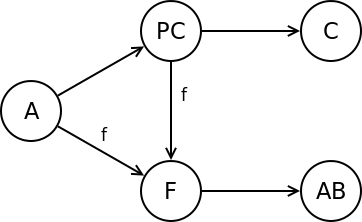
\includegraphics{stavy}}
				\end{figure}
				
				\begin{itemize}
					\item \textbf{Aktivní (A)} -- počáteční stav, transakce v něm setrvává po dobu provádění
					\item \textbf{Částečně potvrzená (PC)} -- po provedení posledního příkazu
					\item \textbf{Chybový stav (F)} -- po zjištění, že normální provádění není dál možné
					\item \textbf{Zrušená (AB)} -- poté, co byly změny v databázi provedené transakcí anulovány (operace rollback), databáze bude vestavu před zahájením transakce
					\item \textbf{Potvrzená (C)} -- po úspěšném dokončení transakce
				\end{itemize}
			\end{itemize}

			\subsubsection{Uspořádané plány}
				Binární relace "je v konfliktu" z množiny instrukcí transakce $\textrm{T}_{\textrm{i}}$ do množiny instrukcí souběžné transakce $\textrm{T}_{\textrm{j}}$
				\begin{table}[h!]
					\center
					\begin{tabular}{ c  c  c }
						\begin{minipage}{.3\textwidth}
							\centering
							\scalebox{0.5}{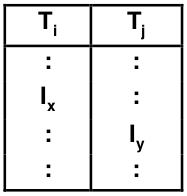
\includegraphics{imgs/tab1_usp_plan}}
						\end{minipage}
						& $\textrm{I}_{\textrm{x}}$ je v konfliktu s $\textrm{I}_{\textrm{y}}$ &
						\begin{minipage}{.3\textwidth}
							\centering
							\scalebox{0.4}{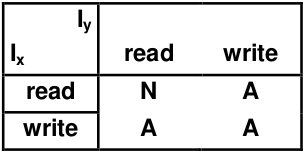
\includegraphics{imgs/tab2_usp_plan}}
						\end{minipage}
					\end{tabular}
				\end{table}
				
			\subsubsection{Graf relace precedence transakcí}			
				Je graf reprezentující binární relaci ''$T_i$ předchází $T_j$'' implikovanou konfliktními instrukcemi transakci $T_i$ a $T_j$.
				Plán je uspořádatelný vzhledem ke konfliktům právě, když je odpovídající graf precedence acyklický.

				\begin{figure}[h!]
					\centering
					\scalebox{0.5}{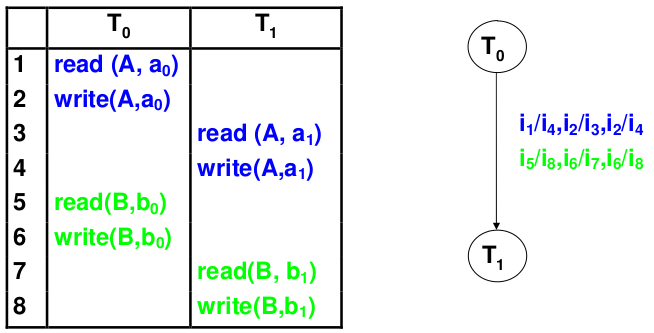
\includegraphics{imgs/acyklicky-graf}}
				\end{figure}
				\begin{figure}[h!]
					\centering
					\scalebox{0.5}{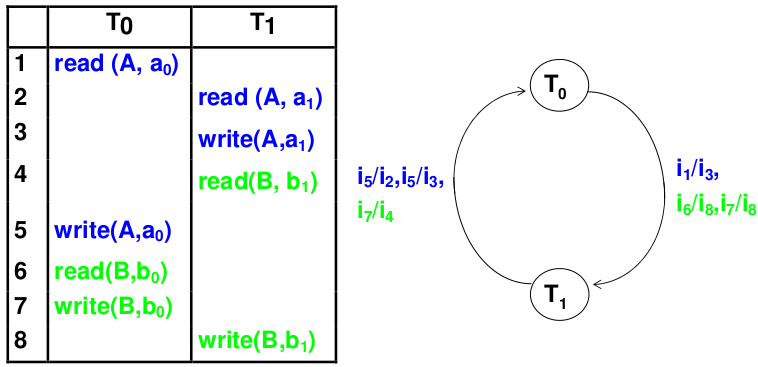
\includegraphics{imgs/cyklicky-graf}}
				\end{figure}
				\pagebreak			
				
			\subsubsection{Plány}
				\begin{itemize}
					\pojem{Plán souběžných transakcí (schedule)}{Chronologické pořadí provádění databázových operací \texttt{read} a \texttt{write} souběžně probíhajících transakcí. Označuje se také jako rozvrh souběžných transakcí}

					\pojem{Uspořadatelný vzhledem ke konfliktům}{Plán souběžných transakcí S se nazývá uspořádatelný vzhledem ke konfliktům, jestliže existuje sériový plán ekvivalentní s plánem S vzhledem ke konfliktům}

					\pojem{Uzamykací protokoly}{Soustava pravidel určující, kdy může transakce zamknout/odemknout objekt}
					\begin{itemize}
						\pojem{Sdílený zámek}{může s ním pracovat více transakcí}
						\pojem{Výlučný zámek}{používá max jedna transakce, která má k objektu výlučný přístup}
					\end{itemize}

					\pojem{Dvoufázový uzamykací protokol}{zajišťuje uspořadatelnost vzhledem ke konfliktům, ne však deadlock}
					\begin{itemize}
						\pojem{Fáze růstu}{transakce uzamyká objekty podle potřeby, ale neodemyká je (uzamykací kód)}
						\pojem{Fáze zmenšování}{transakce odemyká objekty, ale už žádný nesmí zamknout}
					\end{itemize}

					\pojem{Implementace uzamykání}{správce uzamykání používá tabulku zámků (hašovaná tabulka)}

					\pojem{Granularita uzamykání}{Udává jak velká část DB podléhá uzamykání (řádky, blok, atd.)}

					\pojem{Deadlock}{Stav systému kdy žádná z transakcí nemůže pokračovat, protože jí v tom brání jiná transakce (typicky při uvolňování zdrojů -- zámků)}
					\begin{itemize}
						\pojem{Řešení}{protokol zabraňující deadlocku nebo timeout}
					\end{itemize}
				\end{itemize}

				\subsubsection{Řízení souběžného přístupu}
				\begin{itemize}
					\item Problémy při souběžném přístupu:
					\begin{itemize}
						\item Ztráta aktualizace
						\item Závislost na potvrzení načtené hodnoty
						\item Přepis nepotvrzené hodnoty
						\item Nekonzistentní analýza
					\end{itemize}
					\pojem{Schéma řízení}{souhrn pravidel použitých k zajištění souběžného přístupu}
					\pojem{Plán (rozvrh)}{udává chronologické pořadí provádění instrukcí souběžných transakcí}
					\pojem{Sériový plán}{instrukce jedné transakce bezprostředně za sebou}
				\end{itemize}
				\begin{figure}[h!]
					\centering
					\scalebox{0.7}{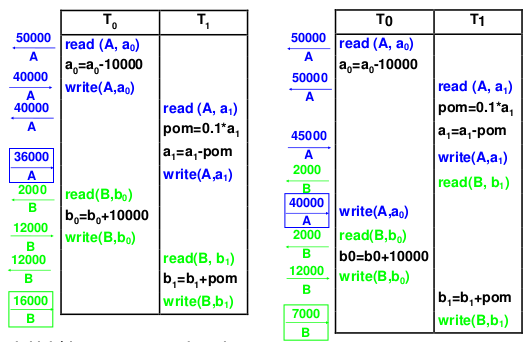
\includegraphics{imgs/Seriovy-plan}}
				\end{figure}
				Obrázek demonstruje správný seriový plán vlevo a špatný vpravo. Je nutné zachovat postup čtení z proměnných v době, kdy je už změnil jiný plán.
				\begin{table}[h]
					\center
					\begin{tabular}{| c | c | c |}
						\hline
						\textbf{Ztráta aktualizace} &
						\textbf{Závislost na potvrzení načtené hodnoty} &
						\textbf{Přepis nepotvrzené hodnoty} \\ \hline \hline
						\begin{minipage}{.3\textwidth}
							\centering
							\scalebox{0.8}{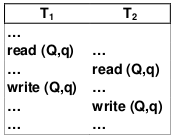
\includegraphics{imgs/ztr_akt}}
						\end{minipage}
						&
						\begin{minipage}{.3\textwidth}
							\centering
							\scalebox{0.8}{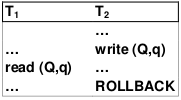
\includegraphics{imgs/zav_pot}}
						\end{minipage}
						&
						\begin{minipage}{.3\textwidth}
							\centering
							\scalebox{0.8}{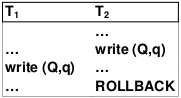
\includegraphics{imgs/prep_nep}}
						\end{minipage}
						\\ \hline
					\end{tabular}
				\end{table}	

		\subsection{Hašování a Indexování}
			\begin{itemize}
				\item Zajištění přístupu k záznamům tabulky podle vybraného sloupce tabulky
				\begin{itemize}
					\pojem{Hašování}{používá hašovací funkci k určení sektoru s daty}
					\pojem{Indexování}{založeno na indexových souborech}
				\end{itemize}

				\pojem{Klíčový atribut}{atribut, který je součástí některého kandidátního klíče}
				\pojem{Kandidátní klíč}{unikátní atribut pro každý řádek tabulky}
				\pojem{Primární klíč}{jeden z kandidátních klíčů, který bude sloužit k adresaci řádků tabulky}
				\pojem{Cizí klíč}{splňuje časově nezávislé vlastnosti:}
				\begin{enumerate}
					\item Každá hodnota FK je buď plně zadaná nebo plně nezadaná
					\item Existuje relace R s kandidátním klíčem CK takovým, že každá zadaná hodnota FK je identická s hodnotou CK nějaké n-tice relace R
				\end{enumerate}
				
				\pojem{Uspořádaný index}{datová struktura tvořená záznamy obsahujícími hodnoty vyhledávacího klíče}

				\pojem{Primární index}{index pro primární vyhledávací klíč}

				\pojem{Sekundární index}{index pro sekundární vyhledávací klíč}

				\pojem{Indexsekvenční soubor}{uspořádaný primární soubor + primární index}

				\pojem{Položka indexu}{záznam obsahující hodnotu vyhledávacího klíče a ukazatele na jeden nebo několik záznamů primárního souboru s touto hodnotou primárního klíče, případně ukazatel na sektor ukazatelů}

				\pojem{Hustý index}{obsahuje položku pro každou hodnotu vyhledávacího klíče, která se v primárním souboru vyskytuje}

				\pojem{Řídký index}{obsahuje jen některé hodnoty vyhledávacího klíče. Takový může být jen primární, protože lze využít uspořádání záznamů v primárním souboru}

				\pojem{Víceúrovňový index}{každá úroveň, s výjimkou poslední, je řídkým primárním indexem úrovně následující. Poslední úroveň je jednoúrovňovým indexem primárního souboru}

				\pojem{Index s unikátními hodnotami (unique index)}{index pro vyhledávací klíč, jehož hodnoty jsou v primárním souboru unikátní}
			\end{itemize}

			\subsubsection{Hašování}
				\begin{itemize}
					\item Hašované soubory $\rightarrow$ přímé hašování
					\item Hašovací funkce převádí hodnotu vyhledávacího klíče na adresu sektoru záznamů

					\item Požadavky na hašovací funkci
					\begin{itemize}
						\item Rozložení hodnot je rovnoměrné
						\item Výskyt hodnot je náhodný
					\end{itemize}

					\item Typické hašovací funkce
					\begin{itemize}
						\item součet bin. reprezentace znaků řetěce \texttt{MOD} počet sektorů
					\end{itemize}

					\item Přetečení sektorů
					\begin{itemize}
						\item Nedostatečný počet sektorů
						\begin{itemize}
							\item[$\circ$] Musí platit $N > \frac{n_z}{z_s}$, kde $N$ je počet sektorů, $n_z$ je celkový počet záznamů a $z_s$ je počet záznamů sektoru
						\end{itemize}
						\item Přetížení některých sektorů (skew)
						\begin{itemize}
							\item[a)] Nerovnoměrné rozdělení hodnot vyhledávacího klíče
							\item[b)] Počet sektorů se volí $\left(\frac{n_z}{z_s}\right)*(1+d)$, kde $d$ je faktor korekce, typicky 0.2 
						\end{itemize}
					\end{itemize}

					\pojem{Hašovaný index}{datová struktura, uspořádaní jejích záznamů je dáno hodnotou hašovací funkce pro hodnotu vyhledávacího klíče obsaženou v daném záznamu}
					\begin{itemize}
						\item Soubor může být hašovaný pouze podle jednoho vyhledávacího klíče
						\item U hašovaného indexu jsou v sektorech položky s hodnotou vyhledávacího klíče a ukazatelem do souboru (obdoba sekundárních indexů)
					\end{itemize}

					\item Nevýhoda statického hašování
					\begin{itemize}
						\item Hašovací funkce se musí zvolit při implementaci, resp. definici hašovaného souboru a nelze ji snadno změnit se změnou velikosti tabulky
					\end{itemize}

					\item Dynamické hašování
					\begin{itemize}
						\item Dynamická modifikace hašovací funkce tak, aby odrážela změny velikosti tabulky
					\end{itemize}
				\end{itemize}

			\subsubsection{Shlukování (clustering)}
				\begin{itemize}
					\item Umístění záznamů se stejnými vlastnostmi (hodnotou klíče pro shlukování) fyzicky blízko u sebe
					\item Přístup k záznamům prostřednictvím indexu nebo hašováním
					\item V souboru mohou být záznamy jedné nebo několika tabulek
				\end{itemize} 
			\subsubsection{Bitmapové indexy}
				\begin{itemize}
					\item Uložení informace o tom, ve kterých záznamech tabulky se vyskytuje daná hodnota vyhledávacího klíče, ve formě bitových vektorů \tedy velikost bitmapového souboru je výrazně menší
					\item Jedničky v bitmapě určují, na kterém řádku se určitý atribut
					\item Pomocí logických operací se nad bitmapami dají vykonávat operace
					\item Př: stejné hodnoty ve dvou tabulkách \\
					\texttt{111110 $\land$ 100101 = 100100}
				\end{itemize}

		\subsection{Pohledy}
			\begin{itemize}
				\item Pojmenovaná virtuální tabulka odvozená z bázové
				\item Definice pohledů se ukládá do systémového katalogu
				\item Při dotazu na pohled se provede transformace nad bázovou tabulkou(zdrojová tabulka z pohledu)
				\item Pohledy s klazulemi \texttt{DISTINCT}, \texttt{GROUB BY}, \texttt{HAVING}, s agregačními funkcemi a spojující několik tabulek umožňují pouze čtení

				\pojem{Materializované pohledy}{výsledek dotazu definujícího pohled je skutečně fyzicky uložen v databázi a je zajištěna aktualizace obsahu}
				\pojem{Selektivní pohled}{obsahuje pouze \texttt{SELECT} a nějaká omezení}
				\pojem{Projektivní pohled (bez pk)}{používá se zde i \texttt{INSERT}}
				\pojem{Projektivní pohled (s pk)}{opět se zde může používat \texttt{INSERT} a navíc sloupce mimo pohled mohou být \texttt{NULL}}
				\pojem{Agregační pohled}{Umožňuje  používání agegačních funkcí a \texttt{INSERT INTO}}
				
				\item Důvody použití \tedy skrytí logické struktury, skrytí složitosti dotazu, skrytí způsobu získávání dat
				\item Deklarace: \texttt{CREATE VIEW pohled AS select}
				\item Příklad: \\ \texttt{CREATE VIEW janska AS SELECT k.* FROM klient k, ucet u} \\
					\texttt{WHERE k.r\_cislo = u.r\_cislo AND u.pobocka = 'Janská'} \\
					\texttt{WITH CHECK OPTION} \\
				\item Výhody: Zpřehlednění práce s daty a sestavování dotazů, velké uplatnění z hlediska ochrany dat
				\pojem{Použití pohledu}
				\begin{itemize}
					\item[a)] Omezení přístupu, skrytí logické struktury (bezpečnost)
					\item[b)] Skrytí složitosti dotazu \tedy zjednodušení
					\item[c)] Skrytí způsobu získání dat \tedy nezávislost na změně dotazu
				\end{itemize}
			\end{itemize}

		\subsection{Kurzor}
			\begin{itemize}
				\item Umožňuje pojmenovat jednotlivé pracovní oblasti a přistupovat k nim
				\item Deklarace: \texttt{DECLARE nazev CURSOR FOR select ORDER BY ...}
				\item Nejčastěji používány v uložených procedůrách a triggerech
				\item Využívají se ve spojení s transakčním rozšířením jazyka SQL
				\item Základní operace: deklarace, otevření a uzavření, přechod na další/předchozí záznam
			\end{itemize}
		\subsection{Databázový trigger}
			\begin{itemize}
				\item Databázový objekt obsahující kód spouštěný specifikovanou událostí v databázi
				\item Databázový trigger je něco jiného než trigger klientské části aplikace, který se spouští typicky událostí formuláře nebo tiskové sestavy
				\item Složky příkazu
				\begin{itemize}
					\item Jméno triggeru
					\item Jméno tabulky \texttt{jmeno [REFERENCING alias\_pro\_OLD\_a\_NEW]}
					\item Čas spuštění akce -- \texttt{BEFORE / AFTER}
					\item Událost -- \texttt{INSERT / DELETE / UPDATE [OF sloupec, ...]}
					\item Spouštěná akce -- \texttt{FOR EACH \{ROW | STATEMENT\} [WHEN podminka] spousteny\_SQL\_prikaz}
				\end{itemize}
				\item Typy databázového triggeru:
				\begin{itemize}
					\pojem{\texttt{BEFORE}}{příkazy těla triggeru se provedou před provedením události, která trigger spouští}
					\pojem{\texttt{AFTER}}{příkazy těla triggeru se provedou po provedení události, která trigger spouští}
					\pojem{Příkazový}{je spuštěn jedenkrát pro příkaz, který způsobí zadanou událost, je-li splněna podmínka uvedená v klauzuli \texttt{WHEN} (když je uvedena)}
					\pojem{Řádkový}{je spuštěn jedenkrát pro každý řádek ovlivněný danou událostí, je-li splněna podmínka uvedená v klauzuli \texttt{WHEN} (když je uvedena)}
				\end{itemize}
				\item Typický použití databázových triggerů
				\begin{itemize}
					\item Implementace integritních omezení
					\item Implementace složitých bezpečnostních omezení (např. možnost modifikace dat jen v určitou dobu)
					\item Implementace auditu (kdo jaké operace prováděl)
					\item Provedení transparentních modifikací při nějaké události
					\item Výpočet hodnot pro sloupec s odvozenými hodnotami
				\end{itemize}
				\item Zásady při použití databázových triggerů
				\begin{itemize}
					\item Použij databázový trigger k zajištění, že při provedení konkrétní operace jsou provedeny odpovídající akce
					\item Použij databázový trigger jen pro centralizované globální operace, které by měly být spuštěny bez ohledu na to, který uživatel/aplikace operací provede
					\item Nepoužívej databázový trigger k odmítnutí nesprávných dat, jestliže lze totéž provést použitím deklarativních integritních omezení
					\item Je-li tělo triggeru rozsáhlé vytvoř uloženou proceduru, která se bude volat z těla triggeru
					\item Nevytvářej rekurzivní triggery
					\item Používej databázové triggery uvážlivě. Provádí se pro každého uživatele/aplikaci pokaždé, když daná událost nastane
				\end{itemize}				
			\end{itemize}
			
		\subsection{Zotavení}
			\begin{itemize}
				\item Znamená obnovení konzistentního stavu databáze po výpadku
				\item Klasifikace výpadku:
				\begin{itemize}
					\pojem{Výpadek transakce}{logická chyba \tedy data nebyly nalezeny nebo systémová chyba \tedy deadlock}
					\item \textbf{Zhroucení systému}
					\item \textbf{Porucha disku}
				\end{itemize}
				\item K zajištění atomicity transakce a trvanlivosti změn je nutné před modifikací databáze uložit do stabilní paměti informace o modifikaci
				\pojem{Žurnál}{posloupnost záznamů žurnálu (log record) zaznamenávající všechny modifikace databáze}
				\begin{itemize}
					\pojem{Start}{začátek transakce}
					\pojem{Commit}{potvrzení, že vše skončilo korektně}
					\pojem{Abort}{transakce byla zrušena}
				\end{itemize}
				\pojem{Archivace}{ukládání obsahu databáze do stabilní paměti}
				\pojem{Obnova}{obnovení databáze do stavu před poslední archivací}
				\item Okamžitá modifikace databáze \tedy umožňuje provádět modifikaci databáze, když je transakce v aktivním stavu. POužívá 2 procedůry:
				\begin{itemize}
					\item UNDO(T$_\textrm{i}$) \tedy pokud dojde k výpadku, vrátí se původní hodnota
					\item REDO(T$_\textrm{i}$) \tedy pokud všechno doběhne korektně, uloží se nová hodnota
				\end{itemize}
			\end{itemize}
			\begin{figure}[h!]
				\centering
				\scalebox{0.65}{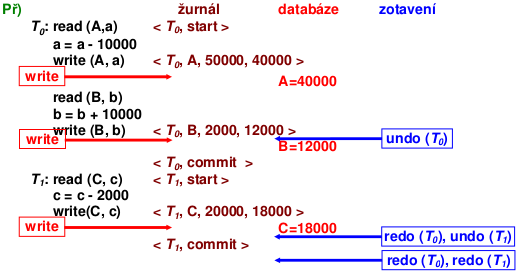
\includegraphics{imgs/Schema-zotaveni}}
			\end{figure}
			\subsubsection{Kontrolní bod (checkpoint)}
				\begin{itemize}
					\item Periodické ukládání vyrovnávacích pamětí žurnálu a databáze na disk z důvodu snížení režie související se zotavením po výpadku
					\pojem{Postup}
					\begin{itemize}
						\item[a)] Uložení všech záznamů žůrnálu z hlavní paměti
						\item[b)] Uložení všech modifikovaných bloků databáze z vyrovnávací paměti na disk
						\item[c)] Uložení záznamu \texttt{<checkpoint>} do stabilní paměti
					\end{itemize}
					\pojem{Schéma zotavení}
					\begin{itemize}
						\item[a)] Nalezení množiny transakcí, které probíhaly nebo byly zahájeny po posledním kontrolním bodu a jejich roztřídění po zotavení
						\item[b)] Aplikace zotavovacích procedur REDO(T$_\textrm{i}$) a UNDO(T$_\textrm{i}$) na každou transakci podle výsledků roztřídění
					\end{itemize}
					\begin{figure}[h!]
						\centering
						\scalebox{0.8}{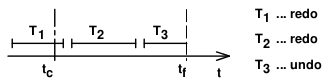
\includegraphics{imgs/Schema-zotaveni-graf}}
					\end{figure}
										
					\pojem{Správa vyrovnávací paměti}
					\begin{itemize}
						\item Datové položky se zapisují přímo na disk -- operace \texttt{write}
						\item Záznamy žurnálu se nezapisují okamžitě do stabilní paměti
					\end{itemize}
					\pojem{Zásady}
					\begin{itemize}
						\item Transakce se dostává do stavu potvrzení až po uložení záznamu \texttt{COMMIT} pro danou transakci stabilní paměti
						\item Před záznamem \texttt{COMMIT} musí být do stabilní paměti uloženy všechny záznamy žurnálu týkající se dané transakce
						\item Před uložením bloku dat do databáze musí být uloženy všechny záznamy žurnálu, týkající se daného bloku \tedy pravidlo WAL (Write-Ahead-Logging)
					\end{itemize}
				\end{itemize}
				

		\subsection{Optimalizace}
			\begin{itemize}
				\pojem{Optimalizace zpracování dotazu}{nalezení (sub)optimální strategie zpracování dotazu, prování SŘDB}
				\item Cílem je min. odezva a max. propustnost
				\pojem{Vstup}{SQL dotaz -- neoptimalizovaný}
				\pojem{Výstup}{plán vyhodnocení, optimální strategie zpracování dotazu}
				\item Přístup k optimalizaci lze založit na statistikách nebo pravidlech
				\item Postup:
				\begin{enumerate}
					\item Převod do vnitřní reprezentace \\
					\texttt{((Klient JOIN Ucet) WHERE mesto = 'Ivančice')[pobocka]}
					\item Nalezení ekvivalentního, ale efektivnějšího výrazu \\
					\texttt{(((Klient WHERE mesto = 'Ivančice')[r\_cislo]) JOIN Ucet)[pobocka]}
					\begin{itemize}
						\item Některá pravidla (heuristiky): \\
						\texttt{(A JOIN B) WHERE podm\_A AND podm\_B = (A WHERE podm\_A) JOIN (B WHERE podm\_B)} \\
						\texttt{(A WHERE podm1\_A) WHERE podm2\_A = A WHERE podm1\_A AND podm2\_A} \\
						\texttt{(A[atributy1])[atributy2] = A[atributy2]} \\
						\texttt{(A[atributy1]) WHERE podm1 = (A WHERE podm1)[atributy1]}
						\item Sémantická optimalizace -- využití sémantické informace \\
						\texttt{(Ucet JOIN Klient)[r\_cislo] = Ucet[r\_cislo]}
					\end{itemize}
					\item Výběr kandidátů procedur pro implementaci operací \tedy statistiky databáze, existence indexů, shlukování, ... 
					\item Generování plánu vyhodnocení a výběr nejlepšího
				\end{enumerate}
			\end{itemize}
			
		\subsection{Integrita databáze}
			\begin{itemize} 
				\item Data v databázi jsou konzistentní vůči definovaným pravidlům
				\item Lze zadávat pouze data, která vyhovují předem definovaným kriteriím
				\item K zajištění integriti slouží integritní omezení
				\begin{itemize}
					\item Jedná se o nástroje, které zabrání vložení nesprávných dat či ztrátě nebo poškození stávajících záznamů v průběhu práce s databází
					\item Je možné zajistit mazání dat, která již ztratila svůj význam 
				\end{itemize}
				\pojem{Referenční integrita}{DB nesmí míst nesouhlasné hodnoty cizího klíče}		
			\end{itemize}
			
			\subsubsection{Druhy integritních omezení}
				\begin{enumerate}
					\pojem{Entitní integritní omezení}{povinné integritní omezení, které zajišťuje úplnost primárního klíče tabulky}
					\pojem{Doménová integritní omezení}{zajišťují dodržování datových typů/domén definovaných u sloupců databázové tabulky}
					\pojem{Referenční integritní omezení}{zabývají se vztahy dvou tabulek, kde jejich relace je určena vazbou primárního a cizího klíče}
					\pojem{Aktivní referenční integrita}{definuje činnosti, které databázový systém provede, pokud jsou porušena některá pravidla}
				\end{enumerate}

			\subsubsection{Dodržování integritních omezení}
				\begin{itemize}
					\item Umístění jednoduchých mechanismů pro dodržování integritních omezení na straně databázového serveru
					\begin{itemize}
						\item Nejlepší způsob z hlediska ochrany dat
						\item Delší odezva systému
						\item Nelze zajistit přenositelnost na jiný DBS
					\end{itemize}
					\item Umístění ochranných mechanismů na straně klienta
					\begin{itemize}
						\item Pro komfort a nezávislost na DBS
						\item Může způsobit chyby u aplikací a v případě většího počtu aplikací je potřeba je opravit na více místech
					\end{itemize}
					\item Samostatné programové moduly na straně serveru
					\begin{itemize}
						\item Použití triggerů \tedy samostatné procedury, které lze spouštět automatizovaně před a po operacích manipulujících s daty
						\item Umožňuje i implementaci složitých integritních omezení
						\item Omezení při provádění na serveru a v přenositelnosti na jiný DBS
					\end{itemize}
				\end{itemize}

		\subsection{Bezpečnost}
			\begin{itemize}
				\item[a)] Důvěrnost \tedy informace by neměly být přístupné neautorizovaným uživatelům
				\item[b)] Integrita \tedy modifikovat data může jen autorizovaný uživatel
				\item[c)] Dostupnost \tedy autorizovaným uživatelům by nemělo být bráněno v přístupu
				\begin{itemize}
					\item Bezpečnostní politika: kdo co může s jakými daty provádět
					\item Bezpečnostní mechanismy: zajištění bezpečnostní politiky
				\end{itemize}	
			\end{itemize}
			\subsubsection{Bezpečnostní mechanismy poskytované SŘBD}
				\begin{itemize}
					\item Pohledy
					\item Řízení přístupu dat
					\begin{itemize}
						\item Nepovinné \tedy založen na přístupových právech, každý uživatel má přístupová práva k databázovým objektům
						\item Povinné \tedy založen na bezpečnostních třídách objektů, stupních prověření subjektů a pravidlech provádění operací
					\end{itemize}
					\item SQL poskytuje podporu pro nepovinné řízení
					\item Typické prostředky pro řízení přístupových práv
					\begin{itemize}
						\item Identifikace uživatelů a rolí (\texttt{CREATE USER, CREATE ROLE})
						\item Přidělování a odnímání přístupových práv (\texttt{GRANT, REVOKE})
						\item Přístupová práva k databázovým objektům
						\item Parametry vztažené k heslu (\texttt{CREATE PROFILE})
					\end{itemize}
				\end{itemize}
		
%%%%%%%%%%%%%%%%%%%%%%%%%%%%%%%%%%%%%%%%%%%%%%%%%%%%%%%%%%%%%%%%%%%%%%%%%%%%%%%%
	\section{Databáze}
		\begin{itemize}
			\pojem{Databáze}{papírová agenda (registr) v podobě perzistentních dat}
			\item Systém pro ovládání souborů:
			\pojem{Nevýhody}
			\begin{itemize}
				\item redundance dat (informace se opakují)
				\item nebezpeční nekonzistence (rozpory v datech)
				\item problémy s přístupem k datům pro neplánové (ad-hoc) dotazy
				\item izolace dat (sbírání dat z jednotlivých souborů)
				\item problémy s bezpečností dat (omezený přístup)
				\item problém integrity (implementace integritního omezení)
			\end{itemize}

			\pojem{Perzistentní data}{data s dobou života překračující běh programu i vypnutí pc}
			\pojem{Další vlastnosti dat v DB}
			\begin{itemize}
				\item Integrovaná \tedy sjednocení do jednoho souboru a odstranění redundance
				\item Sdílená \tedy typicky víceuživatelská (třeba omezeným přístupem)
				\item Bezpečná \tedy shodná realizace omezení přístupu k datům
				\item Snadná integrita (implementace integritních omezení)
			\end{itemize}

			\pojem{Integrita dat}{správnost dat z hlediska splnění omezení (integritních)}
			\pojem{Konzistence dat}{nerozpornost dat \tedy nedojde-li k porušení dat jsou data nekonzistentní}
			\item Systém řízení báze dat (SŘBD) \tedy programová část nad DB (řeší operace)
			\pojem{Databázový systém (DBS)}{systém, který zahrnuje technické prostředky / data DB / SŘBD + aplikační program knihovny, atd. / uživatelé DB}
			\pojem{Základní úrovně abstrakce dat}
			\begin{itemize}
				\pojem{Fyzická (interní) úroveň}{popisuje data, jak jsou skutečně uloženy}
				\pojem{Konceptuální (logická) úroveň}{popisuje data, jak jsou skutečně uloženy a jaké vztahy mezi nimi jsou (vazby)}
				\pojem{Úroveň pohledů (externí)}{popisuje, jak jednotlivá data vnímají jednotliví uživatelé}
			\end{itemize}
			\pojem{Datové modely}{Kolekce konceptuálních nástrojů pro popis objektů, reality, reprezentujících dat, vztahů, sémantiky a integritních omezení}
			\pojem{Rozdělení podle úrovně modelování}
			\begin{itemize}
				\item Logické modely \tedy popisují data na úrovni konceptuální a pohledů -- konceptuální modelování
				\item Databázové modely \tedy definují logickou organizaci v DB
				\item Modely fyzických dat \tedy popisují data na fyzické úrovni
				\item Hierarchický model \tedy záznamy jsou organizovány jako stromy
				\item Síťový model \tedy množina záznamů, pojmenovaných vazeb (obdoba ukazatelů), navigační manipulace s daty
				\item Relační model \tedy na logické úrovni jsou data strukturována do tabulek, manipulace s daty probíhá výběrem z tabulky
				\begin{itemize}
					\item Výhody: technická struktura, jednoduché operace
					\item Nevýhody: informace jsou rozprostřeny po tabulkách, nutno spojovat
				\end{itemize}
			\end{itemize}

			\pojem{Schéma databáze}{metainformace popisující data v databázi, v případě relační databáze obsahuje schéma informace o tabulkách, jejich sloupcích, omezeních na hodnoty ve sloupcích, informace o schématu je typicky uložena v systémovém katalogu}
			\pojem{Datová nezávislost}{schopnost modifikovat schéma bez vlivu na schéma na vyšší vrstvě (úrovni)}
			\begin{itemize}
				\pojem{Fyzická nezávislost}{schopnost modifikace fyzického schématu bez nutnosti přepsat aplikační program}
				\pojem{Logická nezávislost}{schopnost modifikace logického schématu bez nutnosti přepsat aplikační program}
			\end{itemize}
		\end{itemize}
		
			\subsection{Databázové jazyky}
				\begin{itemize}
					\item Jazyk, kterému ''rozumí'' SŘBD, někdy označovány jako databázové
					\item Součástí DB jazyka -- musí existovat prostředky pro:
					\begin{itemize}
						\item Specifikaci schématu databáze \tedy jazyk pro identifikaci dat (DDL $=$ Data Definition Language) -- vytvoří informace v systémovém katalogu (sborníku dat) a dané struktury
						\item Manipulaci s daty \tedy (DML $=$ Data Manipulation Language) -- vyhledávání, modifikace, rušení v daném datovém modelu
					\end{itemize}

					\item Další prostředky
					\begin{itemize}
						\item jazyk pro řízení dat (DCL $=$ Data Control Language) -- transakční zpracování, atd.
					\end{itemize}

					\item Přístup k databázi z aplikačních programů (v čem programujeme)
					\begin{itemize}
						\item používají se speciální databázové jazyky
					\end{itemize}
					
					\item Neprocedurální databázový jazyk
					\begin{itemize}
						\item PL/SQL, Transact SQL, PL/pySQL, Informix 4GL
					\end{itemize}
					\item Obecný programovací jazyk (poskytuje rozhraní pro přístup k DB)
					\begin{itemize}
						\item Naivní \tedy OCi, ADO
						\item Standardizované \tedy ODBC, JDBC
					\end{itemize}

					\item Umožňují začlenit základní DB jazyk do zdrojového textu programu
					\begin{itemize}
						\item SQL pro PASCAL, C, SQLJ pro Javu
					\end{itemize}

					\item Objektově relační mapování \tedy vytváří přístup k virtuální oo databázi
					\begin{itemize}
						\item Hibernate specifikace JDO, JP4a, implementace JPOX
					\end{itemize}
				\end{itemize}

			\subsection{Uživatelé databázových systémů}
				\begin{itemize}
					\pojem{Admin DB}{zajišťuje centrální kontrolu nad daty a programy, mezi funkce patří definice schémat, pamťové struktury a přístupové metody, přidělování práv přístupu, modifikace schématu a fyzické organizace}
					\pojem{Aplikační programátor}{vytváří programy s pomocí jazyků, které manipulují s hostitelskými daty}
					\pojem{Znalý uživatel}{je schopen formulovat požadavky v DB jazyce pro manipulaci s daty}
					\pojem{Naivní uživatel}{komunikuje s programem prostřednictvím aplikace}
				\end{itemize}

			\subsection{Architektura DB systémů a aplikací}
				\begin{itemize}
					\item Datová aplikace ve spojení s SŘBD
					\begin{itemize}
						\item Proces na popředí (fronted, klient) \tedy část aplikace využívající SŘBD
						\item Proces na pozadí (backend, server) \tedy část aplikace realizující věcný základ funkce SŘBD + další funkce (aplikačně orientované)
					\end{itemize}

					\item \emph{Architektura typu ''main frame''}
					\item \emph{Architektura typu ''PC file server''}
					\item \emph{Architektura typu ''Klient/server'' (dvouvrstvá)}
					\item \emph{Vícevrstvá architektura}

					\pojem{V současné době se používají 2 kategorie SŘBD}
					\begin{itemize}
						\pojem{Stolní}{orientované na jednouživatelské aktivity, původně pro architektury file server (Access)}
						\pojem{Serverové}{orientované na víceuživatelské klient/server a vícevrstvé aplikace}
					\end{itemize}

					\pojem{Typy DBS}
					\begin{itemize}
						\item Předrelační (hierarchické, síťové)
						\item Relační
						\begin{enumerate}
							\item Architektura typu ''main frame'' \tedy systémy v 2. pol. 20. let
							\item Architektura typu ''PC file server'' \tedy FOXBASE
							\item Architektura typu ''Klient/server'' (dvouvrstvá) \tedy ORACLE SQL, Microsoft SQL
						\end{enumerate}
						\item Porelační (objektově orientované, objektově relační, deduktivní) \tedy SimpleDB, GemStone
					\end{itemize}
				\end{itemize}

%%%%%%%%%%%%%%%%%%%%%%%%%%%%%%%%%%%%%%%%%%%%%%%%%%%%%%%%%%%%%%%%%%%%%%%%%%%%%%%%
	\section{SQL\,--\,otázky, příkady}


		\subsection{Hostitelský SQL}
			\begin{itemize}
				\pojem{Charakteristika}{proměnné i sloupce mohou mít stejná jména}
				\item Příkazy mají tvar: \texttt{EXEC SQL sql\_prikaz} a končí středníkem
				\item Proměnné v hostitelském prostředí se značí předponou ':'
				\item Referované hostitelské proměnné musí být definovány v deklarační sekci
			\end{itemize}
		\subsection{Dynamický SQL}
			\begin{itemize}
				\pojem{Charakteristika}{poskytuje možnost vytváření příkazů SQL jako textových řetězců za běhu}
				\item Příklad použití:
				\begin{itemize}
					\item Vytvoření příkazu: \\ \texttt{PREPARE jméno\_příkazu FROM řetězec/proměnná}
­ 					\item Vykonání příkazu: \\ \texttt{EXECUTE jm\_příkazu [INTO ...][ USING vstupní\_hodnoty]}
­ 					\item Uvolnění prostoru: \\ \texttt{DEALOCATE PREPARE jm\_příkazu}
					\item Vytvoření příkazu a bezprostřední provedení: \\ \texttt{EXECUTE IMMEDIATE řetězec|proměnná}
				\end{itemize}
			\end{itemize}

		\subsection{Procedury v prostředí Oracle}
		\begin{verbatim}
		CREATE OR REPLACE PROCEDURE jméno(jméno_proměnné TYP_PROMĚNNÉ) 
		BEGIN
		    tělo procedury
		END;	
		\end{verbatim}

		\subsection{Funkce v prostředí Oracle}
		\begin{verbatim}
		CREATE OR REPLACE FUNCTION jméno(jméno_proměnné TYP_PROMĚNNÉ) 
		    RETURN NUMBER
		    IS jméno NUMBER(specifikace)
		BEGIN
		    tělo funkce + return
		END;
		\end{verbatim}

		\subsection{Triggery v prostředí Oracle}
		\begin{verbatim}
		CREATE OR REPLACE TRIGGER jméno
		    [BEFORE|AFTER|INSTEAD OF][DELETE|INSERT|UPDATE|OR]
		    FOR EACH ROW
		BEGIN}
		    tělo procedury
		END;
		\end{verbatim}

%%%%%%%%%%%%%%%%%%%%%%%%%%%%%%%%%%%%%%%%%%%%%%%%%%%%%%%%%%%%%%%%%%%%%%%%%%%%%%%%
	\section{Normalizace}
		\subsection{Teorie závislostí}
			\begin{itemize}
				\pojem{Funkční závislost}{hodnota atributu relace určuje jednoznačně hodnotu jiného atributu téže relace}
				\begin{itemize}
					\item Zapisujeme $X \rightarrow Y$
					\item Vyplývá z významu atributů, představuje integritní omezení
					\item \emph{Nechť X a Y jsou atributy relace R. Řekneme, že Y funkčně závisí na X, právě když pro libovolné dvě n-tice t$_1$ a t$_2$ každého přípustného stavu relace R platí, že je-li x$_1$, resp. y$_1$ hodnota atributu X, resp. Y v n-tici t$_1$ a x$_2$, resp. y$_2$ hodnota atributu X, resp. Y v n-tici t$_2$ a x$_1 = $ x$_2$, potom i y$_1 = $y$_2$.}
					\item Praktický důsledek: opakuje-li se v relaci stejná hodnota determinantu, musí se opakovat i odpovídající stejné hodnoty závislého atributu

					\pojem{Plná funkční závislost}{atribut je funkčně závislý na celém složeném atributu a není funkčně závislý jen na některé jeho části}
					\item Je-li kandidátní klíč relace složený, stejné hodnoty složek se mohou opakovat \tedy musí se opakovat i hodnoty atributů, které jsou částečně (ne plně) závislé
				\end{itemize}
				\pojem{Tranzitivní závislost}{atribut je funkčně závislý na jiném funkčně závislém atributu}

				\item Návrh databáze:
				\begin{itemize}
					\item Proces návrhu založený na teorii závislostí se nazývá normalizace
					\item Postup návrhu: seznam atributů $\rightarrow$ postupná dekompozice na schéma v dostatečně vysoké normální formě
					\item Praktický postup: datový model $\rightarrow$ transformace na schéma relační databáze $\rightarrow$ zjemnění využitím normalizace resp. normalizace ER modelu před transformací
					\pojem{Problémy špatného návrhu}
					\begin{enumerate}
						\item Opakující se informace (redundance)
						\item Nemožnost reprezentovat určitou informaci
						\item Ztráta informace
						\item Složitá kontrola integritních omezení
					\end{enumerate}
				\end{itemize}	
			\end{itemize}
			\subsubsection{Normalizace\,--\,popis}
				\begin{itemize}
					\item Postupná transformace tabulky do vhodnějšího tvaru (postupná dekompozice)
					\item Žádoucí vlastnosti dekompozice:
					\begin{itemize}
						\pojem{Bezeztrátovost při zpětném spojení (Loosless-Join/Nonloss decomp.)}{spojení tabulek, které vzniknou dekompozicí musí dát přesně původní tabulku}
						\pojem{Zachování závislostí}{všechny původní závislosti musí být zachovány a snadno kontrolovatelné (v rámci jedné tabulky)}
						\pojem{Odstranění opakování informace (redundance)}
					\end{itemize}
					\pojem{Boyce-Coddova normální forma (BCNF)}
					\begin{itemize}
						\item Odstraňuje opakování informace
						\item Všechny netriviální funkční závislosti jsou dány závislostí na kandidátních klíčích
						\item Ne každá dekompozice do BCNF zachovává závislosti \tedy potom stačí 3NF
					\end{itemize}
				\end{itemize}

		\subsection{Normální formy}
			\begin{itemize}
				\item Definuje požadavek na vlastnosti schématu relace z pohledu závislostí mezi atributy
				\item Hierarchie normálních forem (Codd: 1NF až 3NF, BCNF, 4NF, 5NF), tj, n-tá normální forma musí splňovat podmínky (n-1) normální formy a něco navíc
				\item Požadavky na návrh založený na normalizaci:
				\begin{itemize}
					\item Bezeztrátovost dekompozice
					\item Zachování závislostí
					\item Dosažení minimálně BCNF, resp. 3NF
				\end{itemize}
				\item Terminologie:
				\begin{itemize}
					\item Klíčový atribut \tedy atribut, který je součástí kandidátního klíče
					\item Superklíč \tedy nadmnožina kandidátního klíče
				\end{itemize}
			
				\item \textbf{První normální forma \texttt{1NF}} \hfill {\small (atomické prvky)}
				\begin{itemize}
					\item relace je v první normální forme, právě když \emph{všechny její jednoduché domény obsahují pouze atomické hodnoty}
				\end{itemize}

				\item \textbf{Druhá normální forma \texttt{2NF}} \hfill {\small (vazba ven z kandidátního klíče)}
				\begin{itemize}
					\item schéma relace je ve druhé normální formě, právě když je v 1NF a \emph{každý její neklíčový atribut je \underline{plně} funkčně závislý na každém kandidátním klíči}
				\end{itemize}

				\item \textbf{Třetí normální forma \texttt{3NF}} \hfill {\small (tranzitivnost)}
				\begin{itemize}
					\item schéma relace se ve třetí normální formě, právě když je ve 2NF a \emph{neexistuje žádný neklíčový atribut, který je tranzitivně závislý na některém kandidátním klíči}
				\end{itemize}

				\item \textbf{Boyce-Coddova normální forma \texttt{BCNF}}
				\begin{itemize}
					\item schéma relace je v Boyce-Coddově normální formě, jestliže \emph{pro každou netriviální funkční závislost $X \rightarrow Y$ je $X$ superklíčem}
				\end{itemize}

				\item \textbf{Čtvrtá normální forma \texttt{4NF}}
				\begin{itemize}
					\item vymezuje vlastnosti, které musí splňovat atributy relace s ohledem na vícehodnotové závislosti
				\end{itemize}

				\item \textbf{Pátá normální forma \texttt{5NF}}
				\begin{itemize}
					\item vymezuje vlastnosti, které musí splňovat atributy relace s ohledem na závislosti na spojení
				\end{itemize}
			\end{itemize}

%%%%%%%%%%%%%%%%%%%%%%%%%%%%%%%%%%%%%%%%%%%%%%%%%%%%%%%%%%%%%%%%%%%%%%%%%%%%%%%%
	\section{B+ stromy}
	Dynamická struktura, v uzlech může být ponechán prostor pro další růst s tím, že každý uzel s výjimkou vrcholu je zaplněn minimálně z 50\,\%.
	\begin{itemize}
		\item Více úrovňový index ve tvaru vyváženého n-nárního stromu, kde n je maximální počet následníků
		\item Kořen \tedy minimálně 2 následníci
		\item Listy obsahují n ukazatelů na další
		\item Uzel stromu má typicky velikost jednoho diskového bloku
		\pojem{Sekvenční část}{tvořena položkami indexu, které obsahují hodnotu vyhledávacího klíče a ukazatel do primárního souboru, uzly tvoří jednosměrně vázaný seznam}
		\pojem{Indexová část}{tvoří řídký víceúrovňový index části sekvenční}
		\item Uzel se skládá z n ukazatelů a n-1 hodnot, které určují od-po které hodnoty jsou pod uzly rozdělené
		\item Vytvoření indexu: \\ \texttt{CREATE [UNIQUE] INDEX nazev ON nazev\_bazove\_tabulky(jmeno\_sloupce [ASC|DESC], ...)}
	\end{itemize}

	\begin{figure}[h!]
		\centering
		\scalebox{0.3}{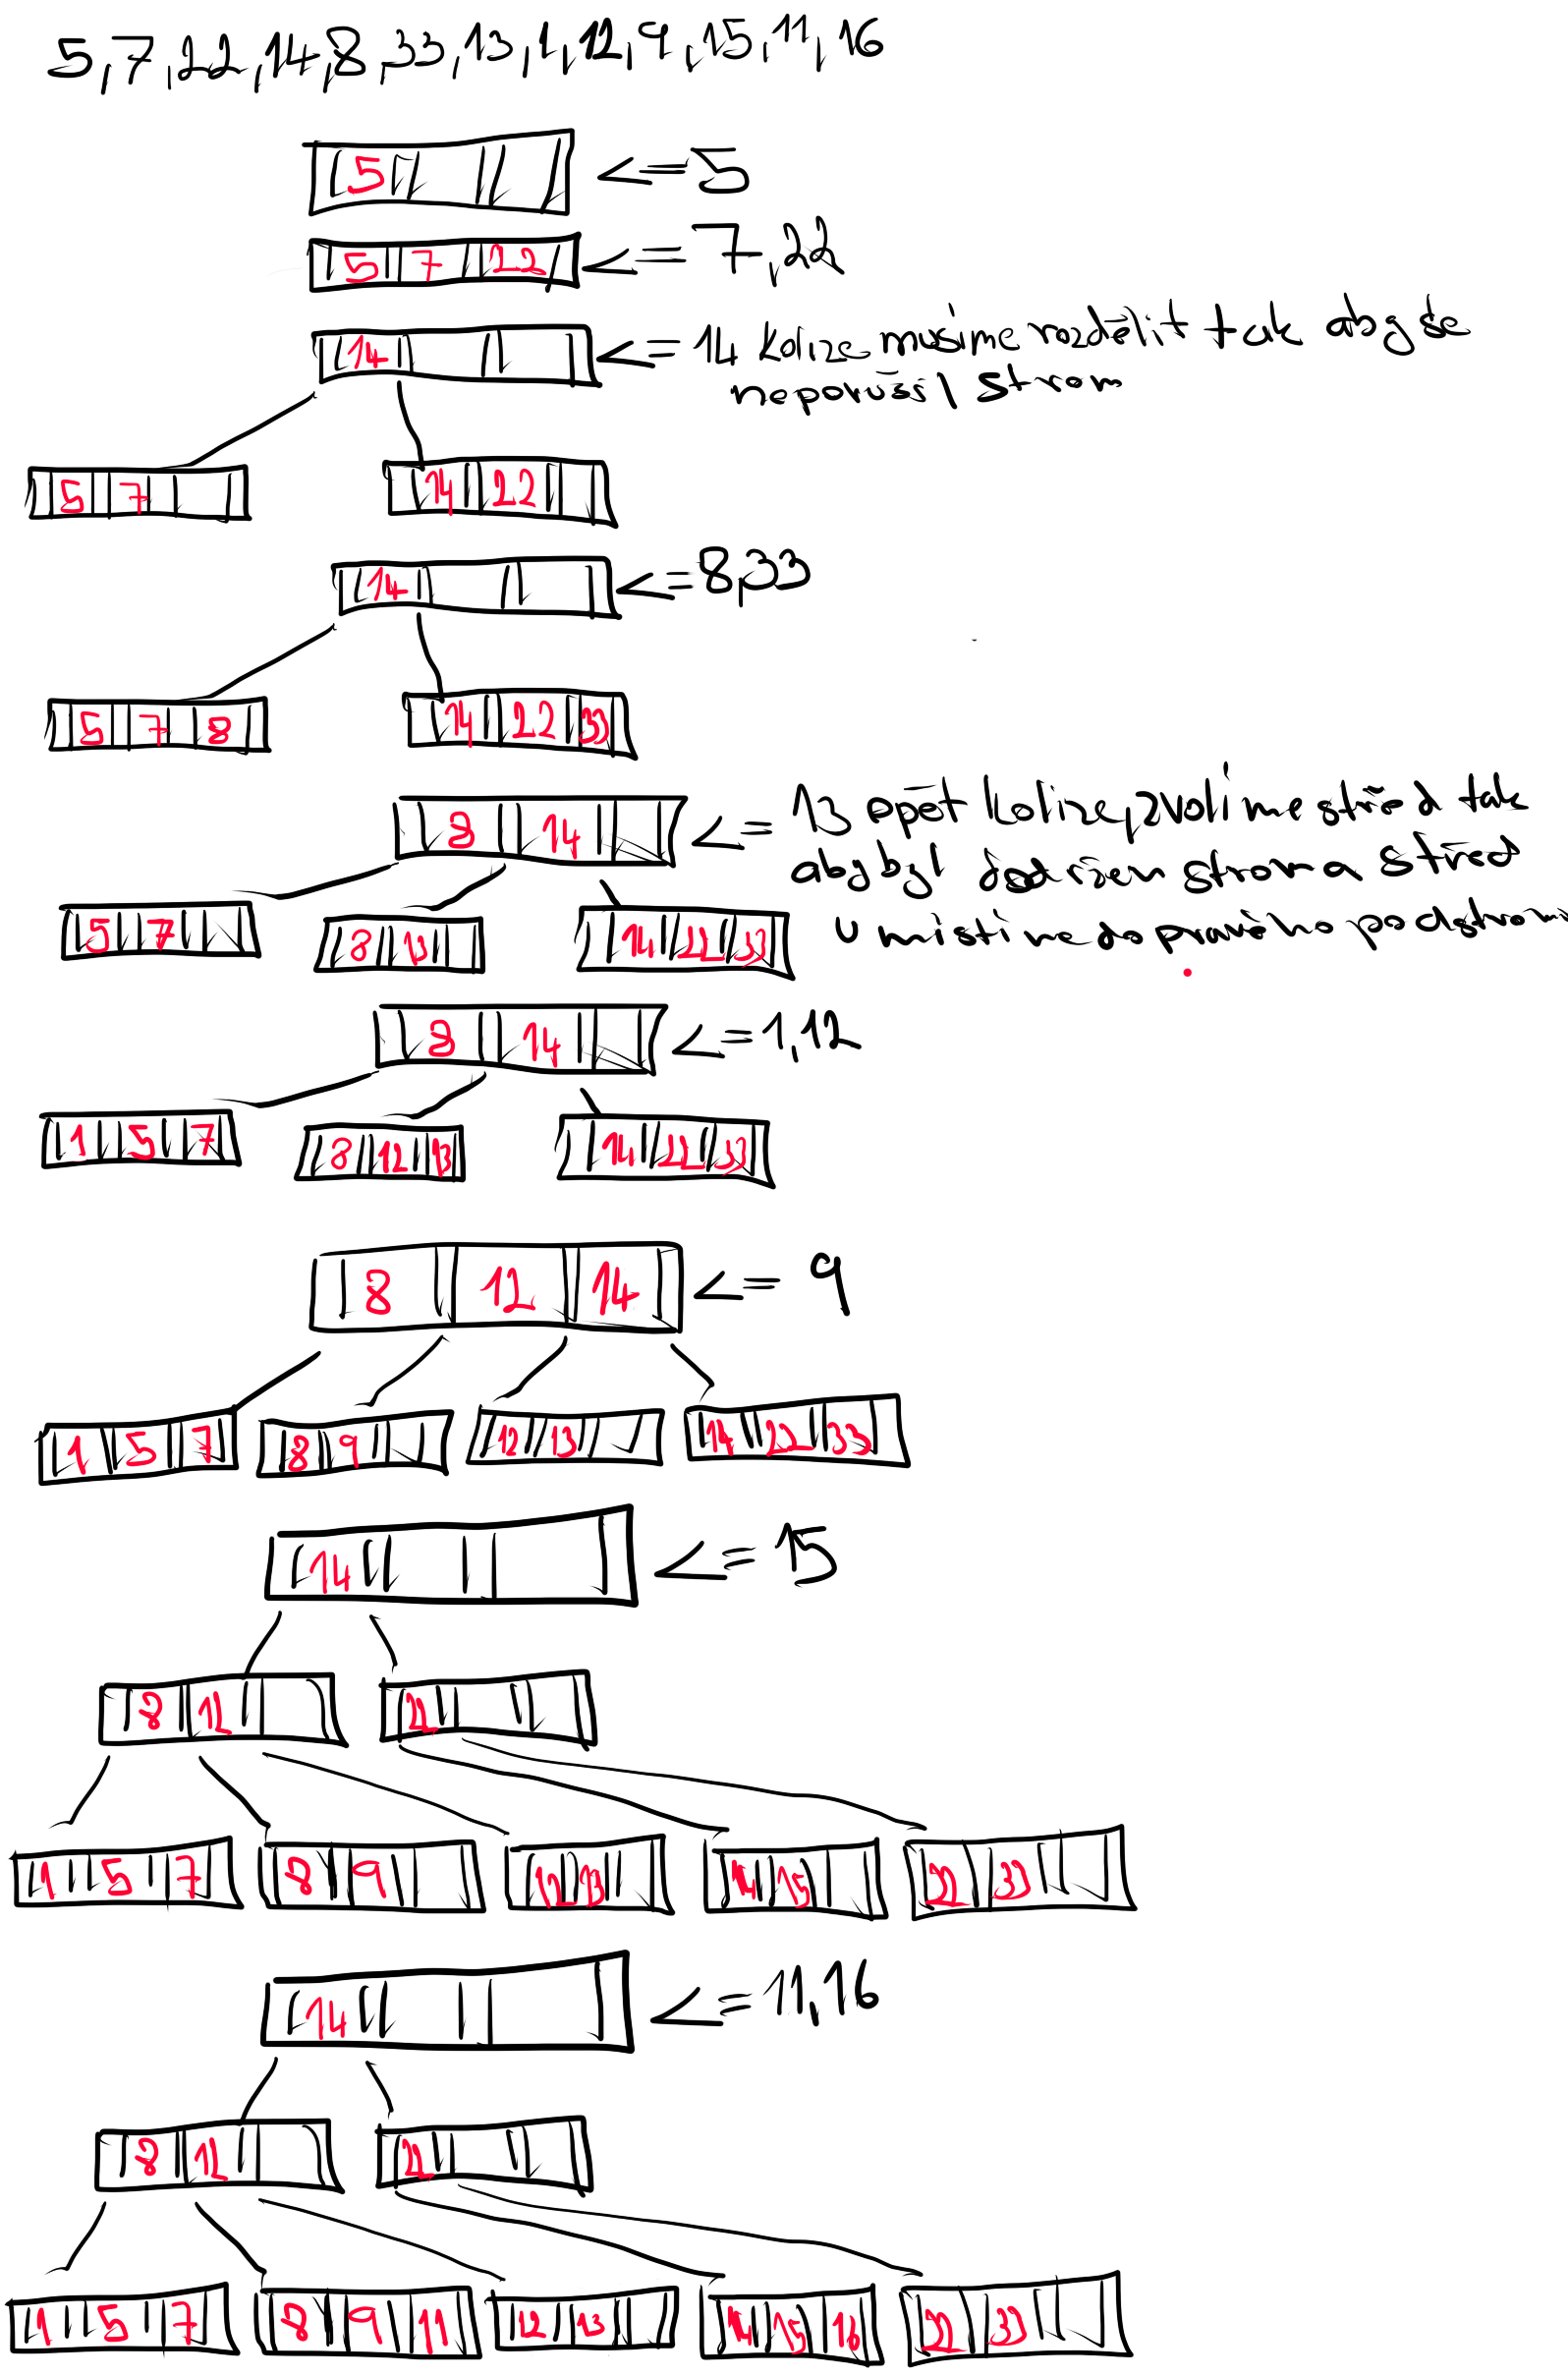
\includegraphics{Bstrom}}
	\end{figure}

			
\end{document}
